\section{Visualizing Time and History}\label{sec:vistime}
\begin{comment}
\begin{itemize*}
  \item Visions of history from the past
  \item Correlated pasts
  \item Non-linear scales
  \item Dynamic/interactive timelines
\end{itemize*}
\end{comment}
\epigraph{What does history look like?  How do you draw time?}{\citet[p. 10]{RosenbergGrafton:2010}}
The questions in this quotation introduce an important topic in the history of data visualization:  how can such a history be visualized? What methods might be invoked to detail the richness of its past?\footnote{Another recent book, \emph{Visualizing Time} \citep{Wills:2012}, discusses a range of  modern graphical methods for visualizing time-based data.} Time provides an obvious dimension, but what else could be included in a static display that might reveal a story previously hidden? What kinds of dynamic or interactive displays might fascinate and intrigue viewers? 

An annotated visual gallery of some timeline designs and visual histories can be found in our Data Visualization Gallery at \url{datavis.ca/gallery/timelines.php}. The topics covered include early visual histories, encyclopedic charts, special purpose charts, correlated histories showing events in one domain in the context of events in other areas, non-linear scales for time and space, as well as dynamic, interactive timelines.  Here we present a few inventive selections from this scholarship.

\subsection{The first timelines, reconsidered}
Although there are earlier precursors, the first timelines of modern design--- featuring a horizontal, linear axis for time, and vertical positions for place, theme or category of events--- were produced in the mid 1700s. Most notable of these prototypes were Jacques Barbeau-Doubourg's 1753 \emph{Carte Chronologique}, and Joseph Priestley's 1765 \emph{Chart of Biography}.

Priestley first published a small ``Specimen'' of this chart as a proof-of-concept, showing the lifespan of famous men in the years 600 BC to 0 AD, classified as ``statesmen'' (from Solon to Augustus) and ``men of learning'' (from Thales to Ovid). Later that year, Priestly published a detailed version \citeyear{Priestley:1765} that quickly became the most popular and influential timeline of the \Cent{19}.  The full graphic details the lifespans of more than 2,000 people from 1200 BC to 1750 AD, classified by their areas of achievement (statesmen \& warriors, mathematicians \& physicians, artists \& poets, and so on).

Priestly's timeline charts can be seen on our Data Visualization Gallery, and we don't reproduce them here.  Instead we show (see \figref{fig:timespan}) a re-design, in his style, of the lifespans of 79 authors from the Milestones database who were born in France or the United Kingdom between 1500 and 2000. 

\begin{figure}[!htb]
  \centering
  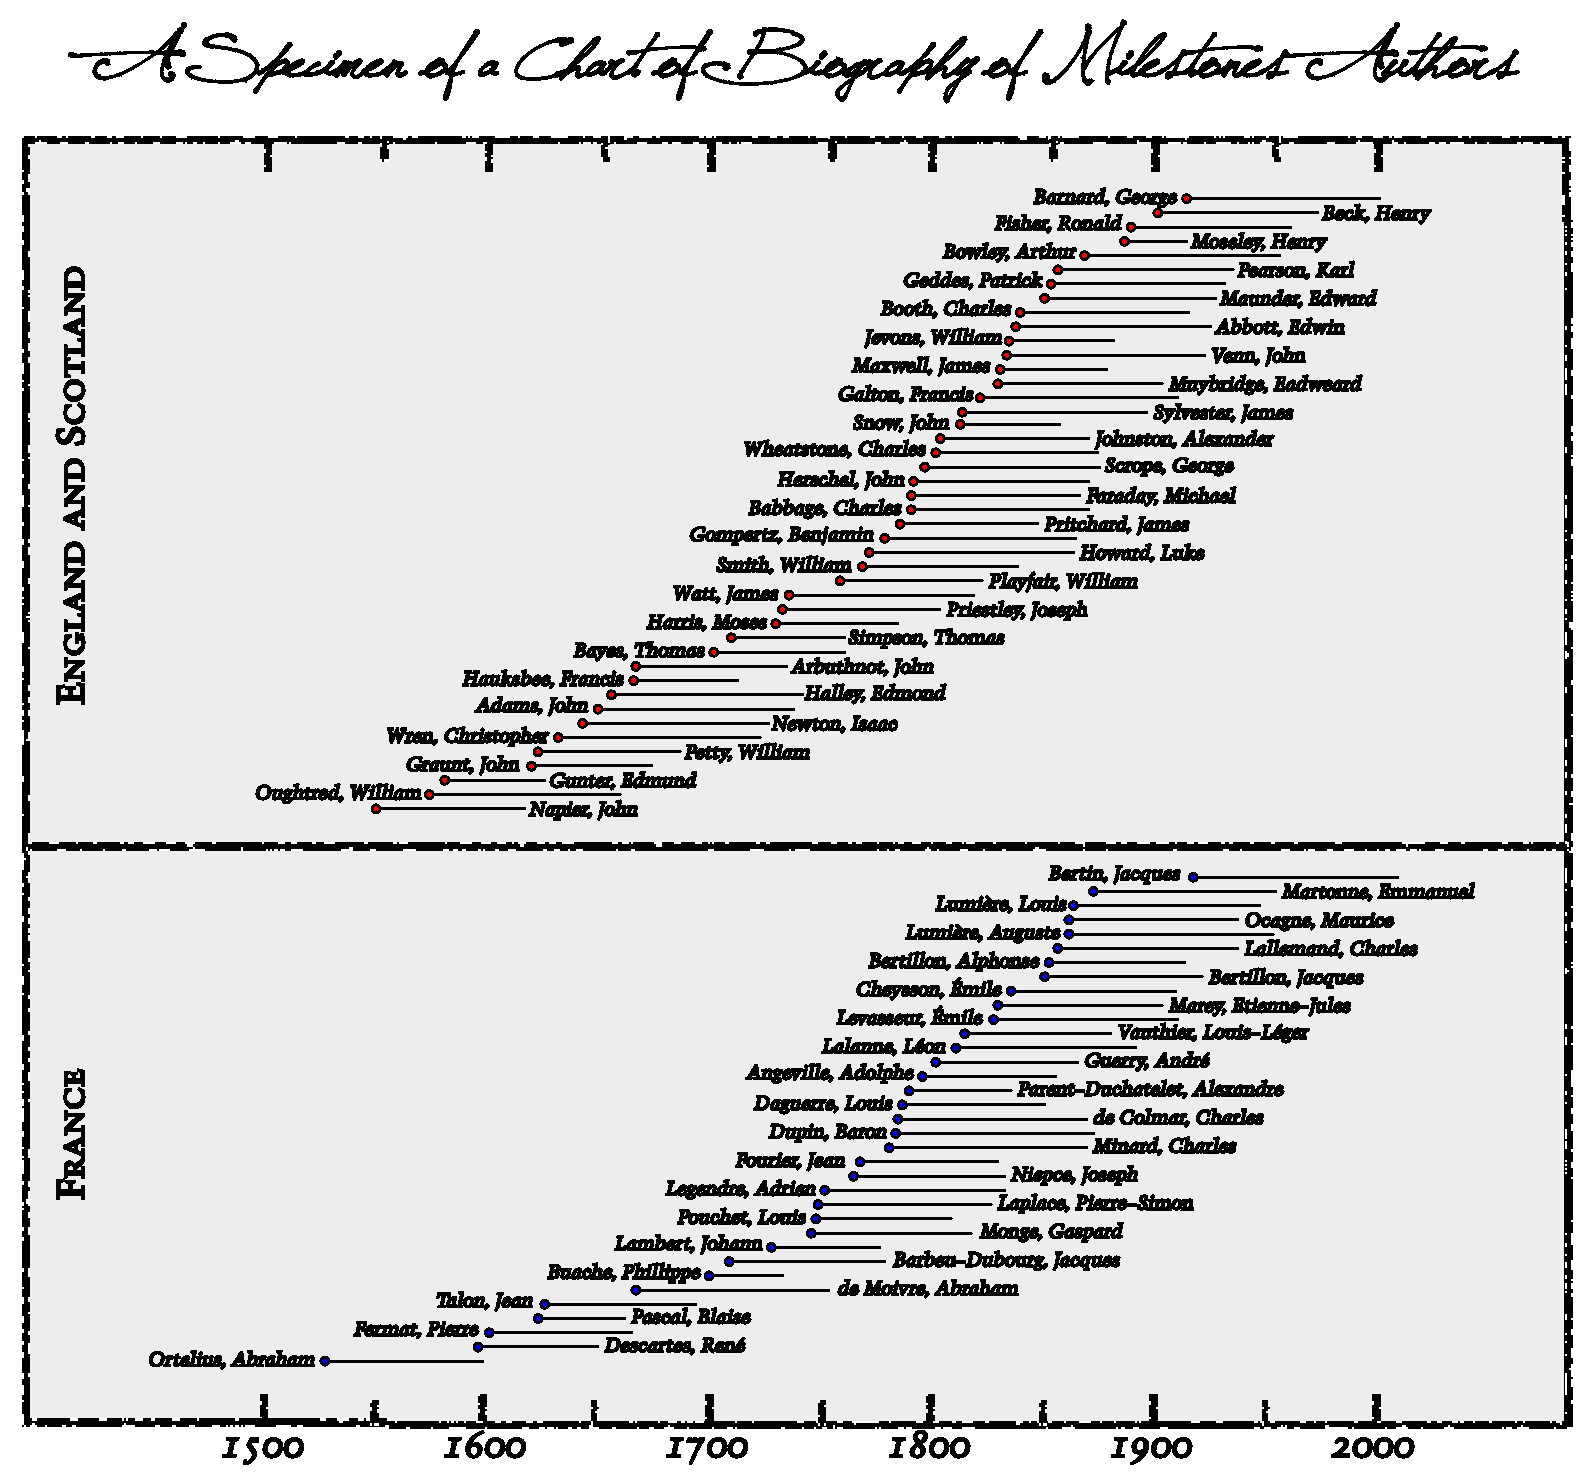
\includegraphics[width=.95\textwidth,clip]{fig/timespan}
  \caption{A modern re-design of Priestley's 1765 \emph{Chart of Biography}, using information on authors in the Milestones database born in France or the United Kindgom. Authors are sorted within country by year of birth and labeled alternately at birth and death years, allowing better lookup and visual comparison.}
  \label{fig:timespan}
\end{figure}

\citet[p. 117]{RosenbergGrafton:2010} called Priestley's charts ``masterpieces of visual economy.'' Indeed, they were at the time.  However, in his charts, the famous people were arranged haphazardly within category groups, so it is difficult to find specific individuals, and nearly impossible to uncover any trends, either over time or across categories. 

In our version, authors are sorted by birth year within each country and the names are printed alternately at the year of birth and death. The result, which resembles a cumulative distribution plot: (a) allows easier visual lookup of names, (b) provides an overall ``lifespan envelope,'' and, (c) highlights a few individuals who lived conspicuously shorter or longer than their contemporaries (e.g., shorter: Willam Jevons,  James Maxwell, John Snow, and Phillipe Buache). Of course, to display lifespan \emph{directly} requires a different kind of plot, but one that would not have been even thinkable by Priestley in 1765.  We return to this question in \secref{sec:lifespan} (see \figref{fig:lifespan}).

\subsection{Universal histories}
%\TODO{Revise figure to include a blowup of a section for greater legibility}
In addition to unrivalled thematic maps and statistical diagrams, the Golden Age of statistical graphics also gave rise to a variety of novel attempts to visualize history in a comprehensive manner, combining parallel, intertwined time-flows, text, illustrations, maps, and other visual forms. Among the most impressive is the series of Synchronological Charts of Universal History produced by Sebastian Adams between 1871--1885. The 1881 version is 23 feet long and captures 5,885 years of history, from 4004 B.C. to 1881 A.D. \citet[p. 172]{RosenbergGrafton:2010} call it ``nineteenth-century America's surpassing achievement in complexity and synthetic power.'' 

\figref{fig:Adams1881} shows just a small portion of the graphic, but the entire chart can be viewed at \url{http://www.davidrumsey.com/blog/2012/3/28/timeline-maps}.  Adams used a linear scale for time, and so it is understandable why it took 23 linear feet to include all of recorded history.

\begin{figure}[!htb]
  \centering
  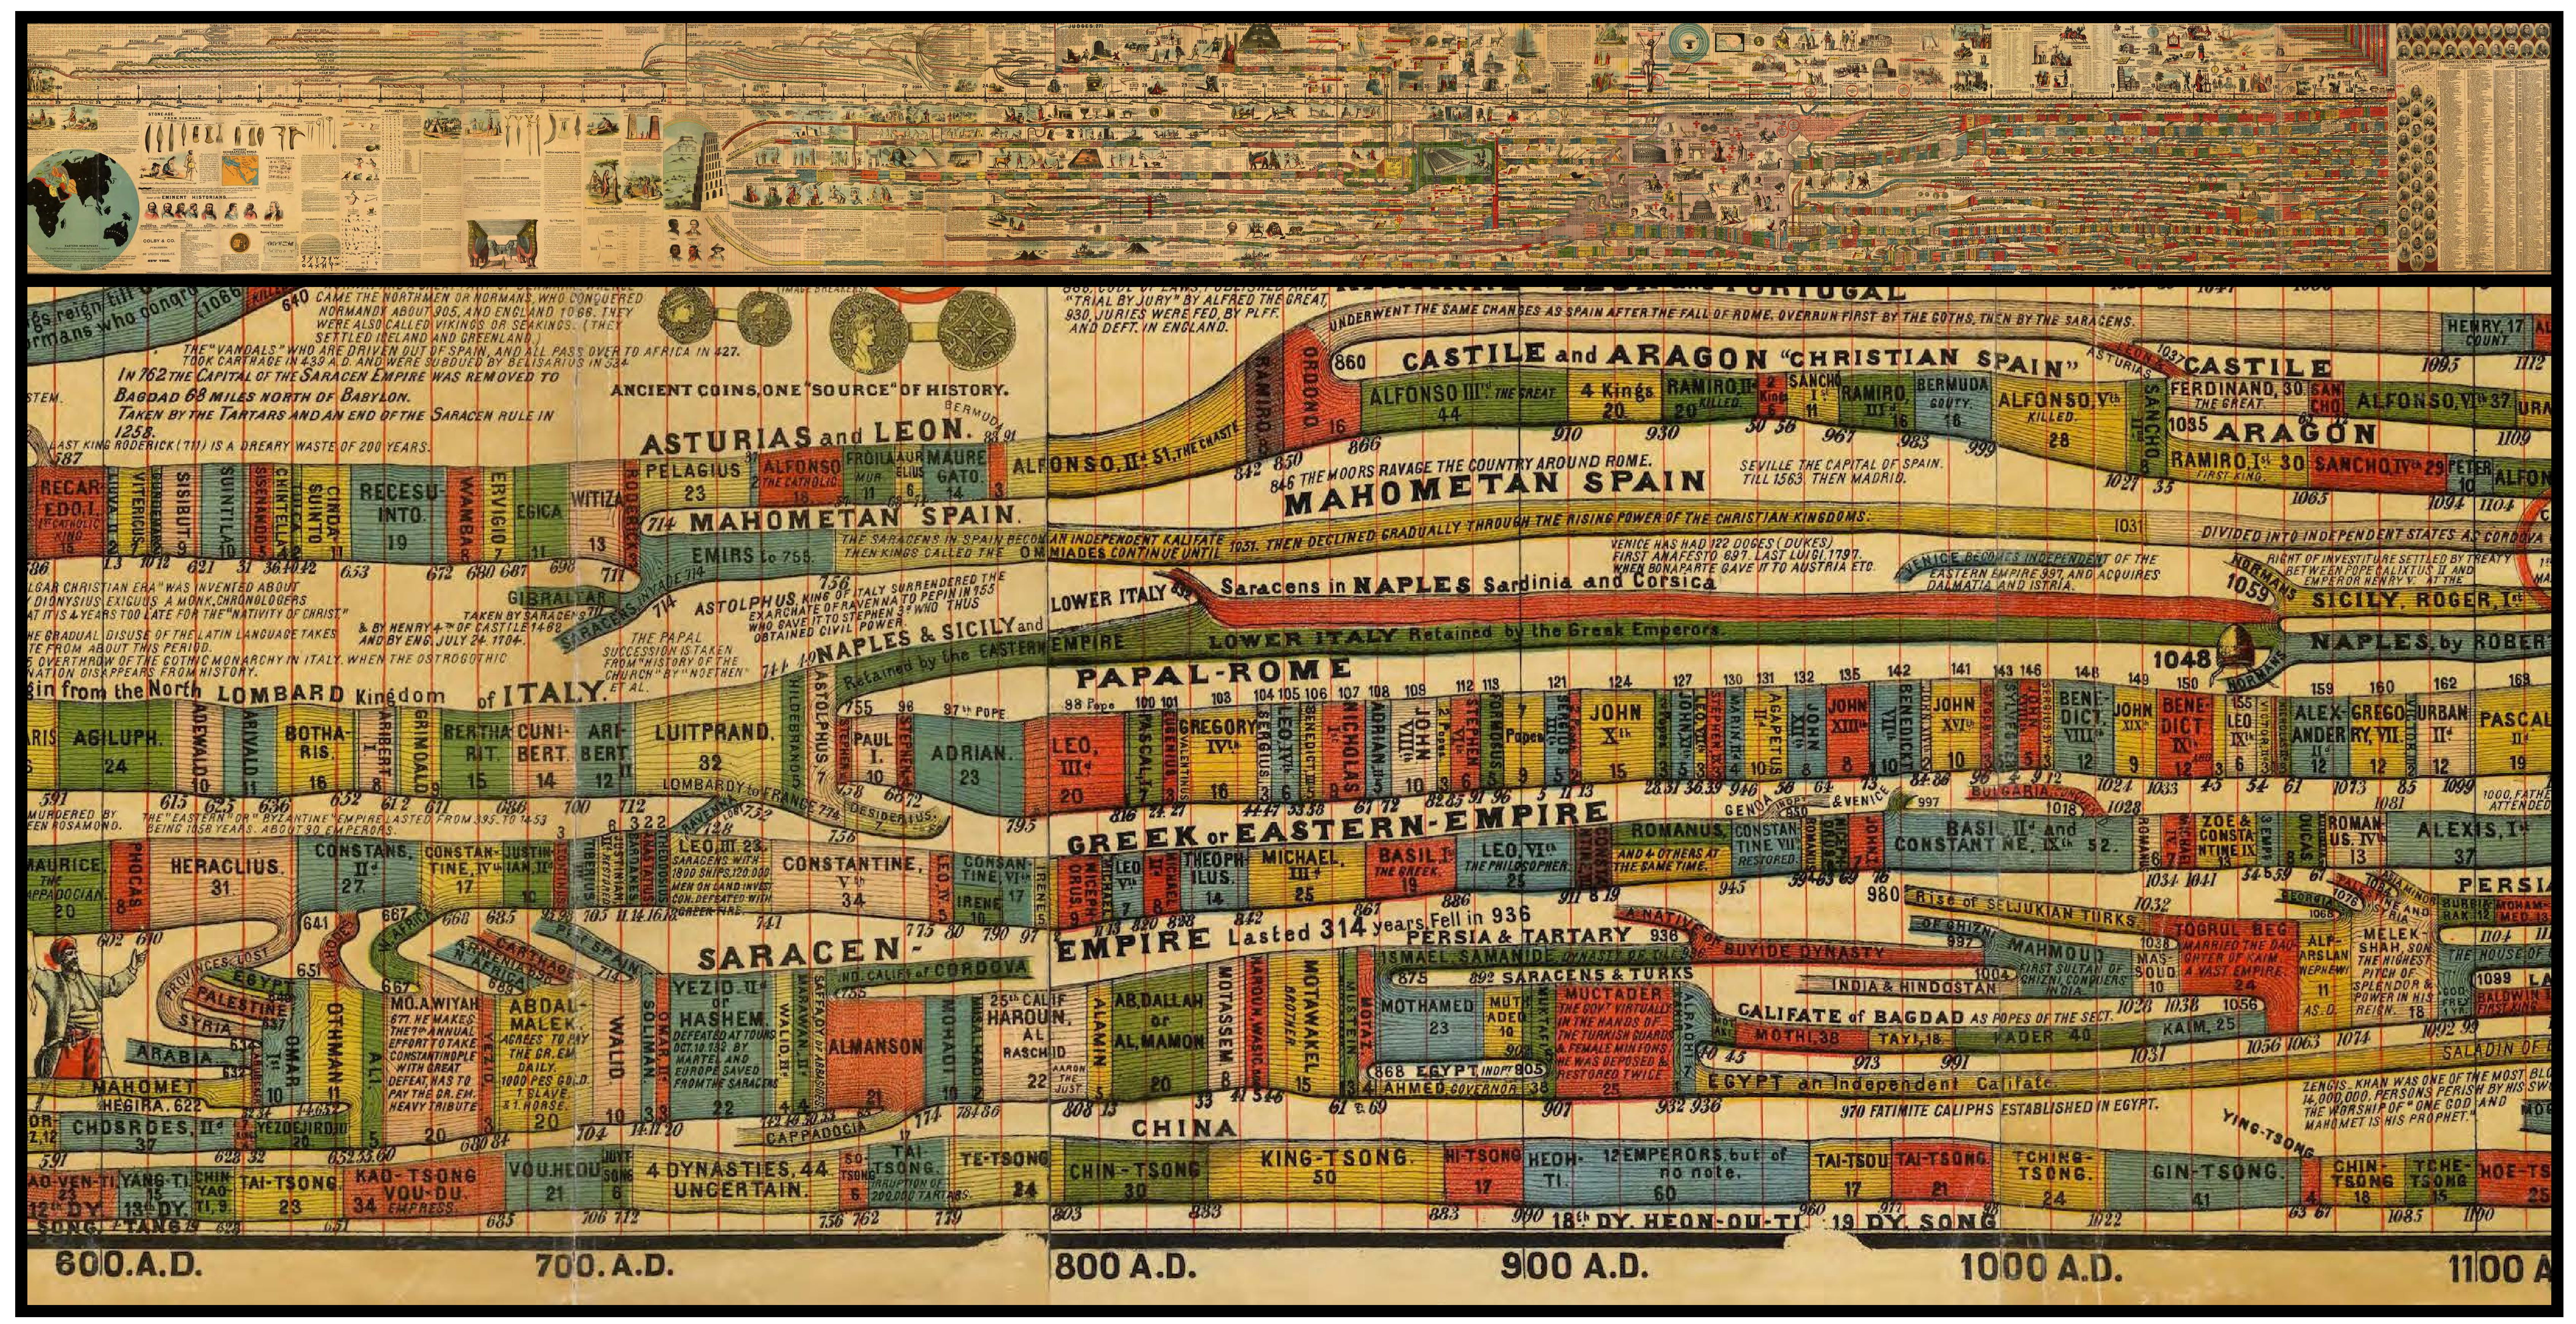
\includegraphics[width=\textwidth,clip]{fig/Adams1881-6}
  \caption{Top: The entirity of Sebastian Adams' \emph{Synchronological Chart of Universal History}, 1881. Bottom: An excerpt detailing the 600--1100AD period. Horizontal bands trace developments in different countries, with detailed text describing significant events, and which break up or merge according to political factors.}
  \label{fig:Adams1881}
\end{figure}

\subsection{Categorization and non-linear scales}
Linear time scales have the advantage that they provide uniform resolution and detail across the entire time span, but events in time, or our interest in them are rarely uniformly distributed. As exemplified by the Milestones Project, most visual histories are rather sparse at their beginning and very crowded at their end. Utilizing non-linear scales can allow resolution to vary smoothly across the range, providing greater detail in regions of interest, which are most often the recent past.

\figref{fig:milecatline} is a proof-of-concept sketch for something that a graphic artist could use as a starting point for a chart of the history of data visualization. It uses the events from the Milestones Project, categorized by two correlated factors: Subject area, in which the content has been categorized as dealing with human populations, physical properties of the world, or mathematics and statistics; and, the milestone's aspect or form, which has been categorized as dealing with cartography, graphs and diagrams, or technology. 

To provide greater resolution for more recent events, we have used a reverse square-root scale going backward from the year 2000. Specifically, `Year' on the horizontal time axis is actually plotted according to the formula $\textrm{Year}^\star = 2* (25 - \sqrt{(2000 - \textrm{Year})})$, giving the more pleasing result that the modern period 1800--2000 occupies about 60\% of the scale, despite only comprising 40\% of the range.  This is subtly observable by the naive viewer through the inspection of the space between the tick marks on the X-axis.

\begin{figure}[!htb]
  \centering
  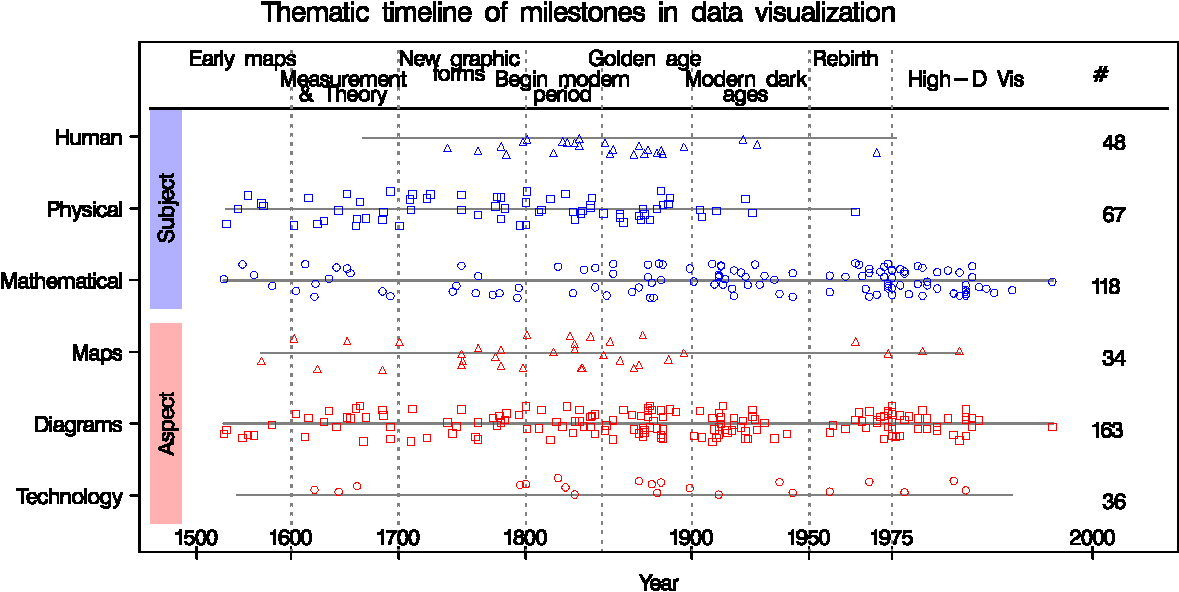
\includegraphics[width=\textwidth,clip]{fig/milecatline}
  \caption{Sketch for a thematic timeline of milestones items, 1500--present, categorized by both the Subject (content) and Aspect (form) of the milestone item.  To provide greater resolution for more recent events, time (Year) is shown on a square-root scale, going backward from the year 2000.}
  \label{fig:milecatline}
\end{figure}